% This example file for NIH submissions was originally written
% by Bruce Donald (http://www.cs.duke.edu/brd/).
%
% You may freely use, modify and/or distribute this file.
%
\documentclass[11pt]{nih_mod}
% last revision:
\def\mydate{2005-06-09 13:58:03 brd}


%%%%%%% Two column control
\newif\ifdotwocol
\dotwocoltrue   % two col
%\dotwocolfalse   % one col
\long\def\twocol#1#2{\ifdotwocol{#1}\else{#2}\fi}
%%%%%%%

\def\mybeforeequation{\footnotesize}
%\def\mybeforeequation{\small}
%\def\mybeforeequation{}

\def\myafterequation{\renewcommand\baselinestretch{1.1}}
%\def\myafterequation{}

%%%%%%%%%%%%%%%%
%%%%%%%%%%%%%%%%

\def\citeusmark{$^{\textstyle \star}$}
\def\citeus#1#2{\cite{#1}}

\def\crow#1#2{#2}

%\usepackage{denselists}
%\usepackage{scaledfullpage}
\usepackage[dvips]{graphicx}
\usepackage[usenames,dvipsnames]{color}
\usepackage[table]{xcolor}
\usepackage{boxedminipage}
\usepackage{amsfonts}
\usepackage{amssymb,amsmath}
\usepackage{url}
\usepackage{setspace}
\usepackage{hyperref}
\usepackage{wrapfig}
%\usepackage[numbers,sort&compress,super]{natbib}
\usepackage[numbers,sort&compress]{natbib}
%\usepackage{times}
%\usepackage{nih}		% PHS 398 Forms
%\usepackage{nihblank}		% For printing on Blank PHS 398 Forms
%\usepackage{confidential}

\definecolor{QNblu}{rgb}{.33,.66,1}
\definecolor{COMPARElightblu}{HTML}{b8c8e5}
\definecolor{COMPAREdarkblu}{HTML}{0055e7}
\definecolor{ECback}{HTML}{c0e0e0}
\definecolor{ECback2}{HTML}{a0c0c0}
\definecolor{ECford1}{HTML}{4080a0}
\definecolor{ECford2}{HTML}{004060}
\definecolor{ECwhite}{HTML}{e0e0e0}


\title{{\bf On reducing transmission risk during conception in serodiscordant couples:} \\ A modeling approach }

\author{Raffaele Vardavas, Glenn Wagner, Deborah Mindry, Risa Hoffman}
\date{}
\begin{document}
\maketitle 

The aim of this project is to develop a mathematical model and produce a deliverable Excel tool that will calculate probabilities of different possible outcomes during conception in serodiscordant couples where the man is HIV+ and woman is HIV-. We will address how PrEP can be used to reduce infection risk. Furthermore by weighting each outcome by an appropriate payoff function we will be able to identify desirable strategies. 


%\pagebreak
\tableofcontents
\pagebreak

\bigskip
\section{Introduction}

We develop a model that predicts the likelihood of possible outcomes defined in terms of HIV infection and successful pregnancy of uninfected women that engage in unprotected sex with infected male partners. These likelihoods depend upon the number of sex acts and the biological parameters that define HIV infectivity (e.g., the male being on treatment or having other STIs) and female fertility (based on age) under different situations.


\section{The Model}

\subsection{The Model Parameters}

The parameters that enter the model are:
\begin{itemize}
	\item $\alpha$: The per unprotected sex act base male to female transmissibility when the male is in the early stage of HIV.
	\item $h_L$: The multiplicative factor that multiples $\alpha$ to provide the per unprotected sex act base male to female transmissibility when the male is in the late stage of HIV.
	\item $h_{Tx}$: The multiplicative factor that multiples $\alpha$ to provide the per unprotected sex act base male to female transmissibility when the male is on HAART.
	\item $h_{STIs}$: The multiplicative factor that multiples $\alpha$ to provide the per unprotected sex act base male to female transmissibility when either partner has other STIs (e.g., genital herpes). 
	\item $h_{PrEP}$: The multiplicative factor that multiples $\alpha$ to provide the per unprotected sex act base male to female transmissibility when the female is taking PrEP.
	\item $p_c(a)$: The probability per unprotected sex act that the female will conceive and become pregnant at age $a$.
	\item $p_d(a)$: The probability that a pregnant female will deliver a baby if she becomes pregnant at age $a$.
	\item $p_{MTCT}$: The probability that an HIV infected (during conception) and pregnant female will infect her baby during pregnancy. 
	\item $h_{TxMTCT}$: The multiplicative factor that multiplies $p_{MTCT}$ to provide the effective mother to child transmission (MTCT) probability when the pregnant female is placed on HAART for the duration of her pregnancy. 
	\item $N$: The number of unprotected sex acts that an uninfected women engages with an infected male partner before being tested again for either pregnancy or HIV status.
\end{itemize}
Thus the overall unprotected sex act base male to female transmissibility is given by:
\begin{equation}
	\tilde{\alpha} = h_{PrEP}\times h_{STIs}\times h_{Tx}\times h_L \times \alpha, 
\end{equation}
where each of the multiplicative factors is taken to be equal to $1$ if the condition does not apply (e.g., $h_L=1$ if the male not in the late stage of HIV). Similarly the effective MTCT transmission is:
\begin{equation}
	\tilde{p}_{MTCT} = h_{TxMTCT}\times p_{MTCT}, 
\end{equation}
where $h_{TxMTCT}$ is taken to be equal to $1$ if the the pregnant female is not on HAART during pregnancy. The probability that the female stays uninfected after $N$ unprotected sex acts is:
\begin{equation}
	[1-\tilde{\alpha}]^N.
\end{equation}
Similarly, the probability that the female never becomes pregnant after $N$ unprotected sex acts is: 
\begin{equation}
	[1-p_c(a)]^N.
\end{equation} 

\subsection{The Model Outcomes}

The are five possible outcomes that are relevant to the female:
\begin{enumerate}
\item  Female stays HIV negative, and becomes pregnant and is successful in giving birth. This occurs with probability:
\begin{equation}
	P_{-\surd} = p_d(a)\{1-[1-p_c(a)]^N\}[1-\tilde{\alpha}]^N.
\end{equation}

\item  Female becomes HIV positive, and becomes pregnant and is successful in giving birth to an HIV negative infant. This occurs with probability:
\begin{equation}
	P_{+\surd - } = p_d(a)(1-\tilde{p}_{MTCT}) \{1-[1-p_c(a)]^N\}\{1-[1-\tilde{\alpha}]^N\}.
\end{equation}

\item  Female becomes HIV positive, and becomes pregnant and gives birth to an HIV+ infant. This occurs with probability:
\begin{equation}
	P_{+\surd +} = p_d(a)\tilde{p}_{MTCT} \{1-[1-p_c(a)]^N\}\{1-[1-\tilde{\alpha}]^N\}.
\end{equation}
\item  Female stays HIV negative, and does not become pregnant. This occurs with probability:
\begin{equation}
	P_{-\times} =  [1-p_c(a)]^N [1-\tilde{\alpha}]^N+[1-p_d(a)]\{1-[1-p_c(a)]^N\}[1-\tilde{\alpha}]^N,
\end{equation}
where the first term represents the case where the female stays HIV negative and does not become pregnant at all and the second term is the probability that she stays HIV negative and does become pregnant but loses the baby before birth. 
\item  Female becomes HIV positive, and does not become pregnant. This occurs with probability:
\begin{equation}
	P_{+\times} =  [1-p_c(a)]^N \{1-[1-\tilde{\alpha}]^N\}+[1-p_d(a)]\{1-[1-p_c(a)]^N\}\{1-[1-\tilde{\alpha}]^N\},
\end{equation}
where the first term represents the case where the female becomes HIV positive and does not become pregnant at all and the second term is the probability that she becomes HIV positive and does become pregnant but loses the baby before birth. 
\end{enumerate}

\subsection{Running the Model}

The model has been constructed in two different platforms: 
\begin{enumerate}
	\item As an Excel tool where users can vary parameter values within given ranges and see a pie chart split by the five outcomes for a given value of $N$ and two further plots showing how these five probabilities change with $N$ (see Figure \ref{Fig:Exceltool}); 
	\item In the statistical software R where we sample the parameters via a Latin Hyper Cube and use these to run many thousands of scenarios (each using a different sampled parameter set) and obtain a sensitivity of the outcomes to each parameter.
\end{enumerate}
\begin{figure}[!h]
  \begin{center}
    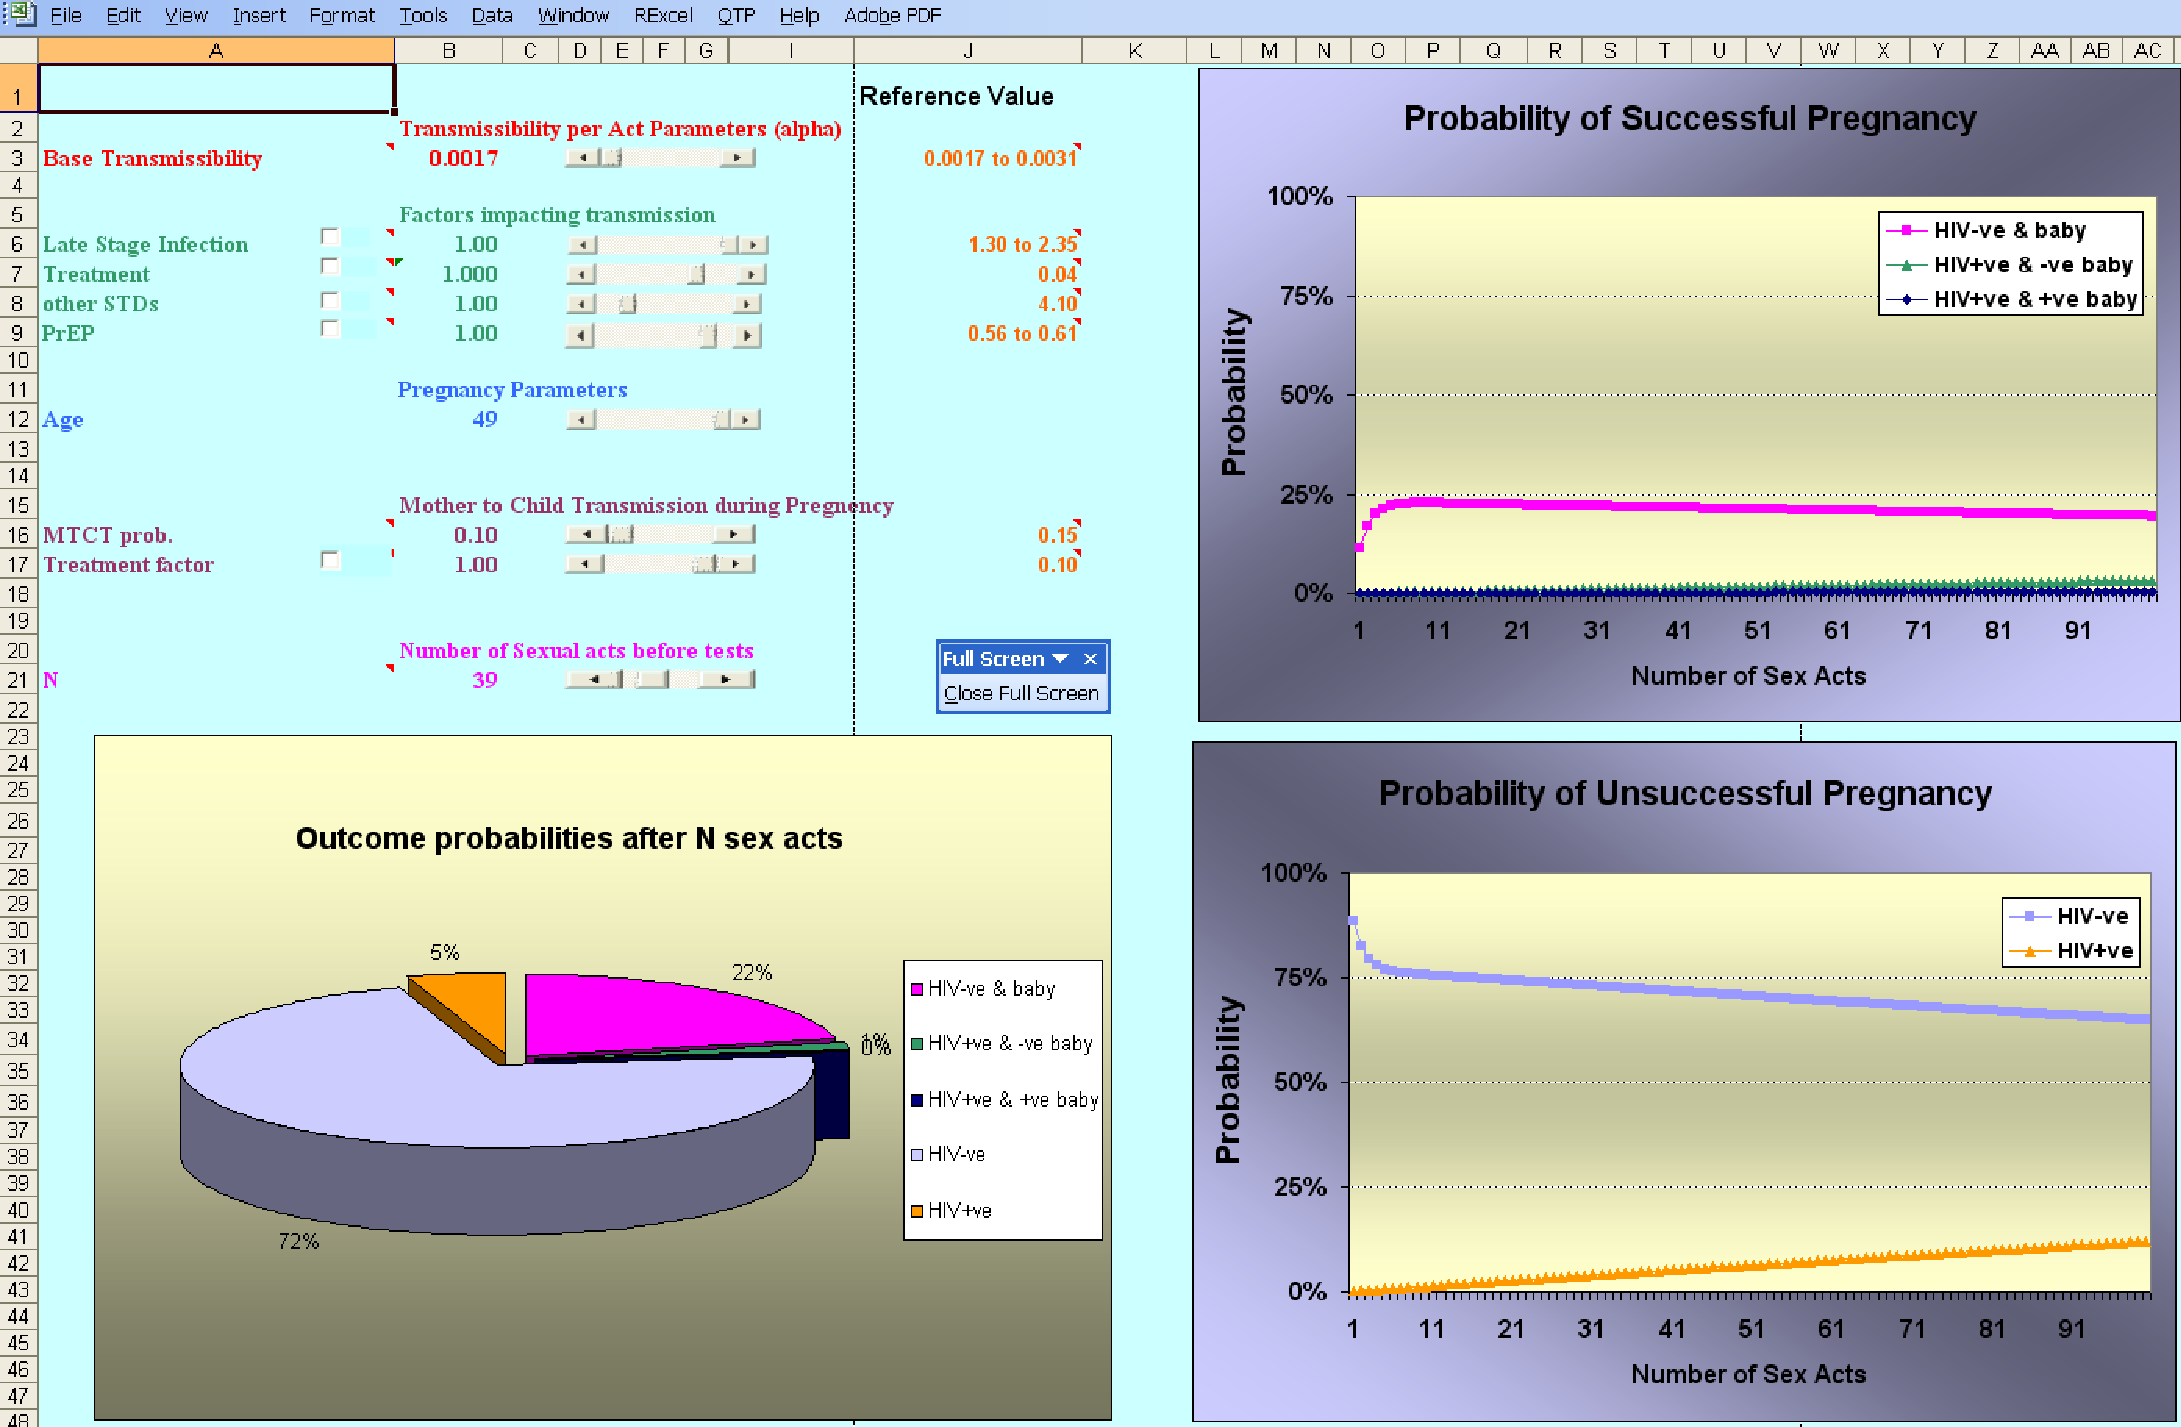
\includegraphics[width=7in]{figures/Exceltool.pdf}
  \end{center}
  \caption{Snap shot of the Excel tool}
  \label{Fig:Exceltool}
\end{figure}
The reference parameters and their ranges are specified similarly in both the Excel tool and the R code. Values for these parameters are described in section \ref{sec:parametes}. When sampling parameters via a Latin Hyper Cube approach we specify a range of values (i.e., a lower and upper bound) and a most likely reference value (the mode). Each parameter may be sampled using different probability distribution functions (pdf). We consider both a Uniform and a beta PERT distribution (see Appendix \ref{sec:PERT}). In the Uniform pdf every parameter value within the range of specified values is equally likely to be selected. In the beta PERT pdf the reference value is a lot more likely to be sampled relative to the boundary values of the parameter range.  


\section{Parameters}
\label{sec:parametes}

Table~\ref{tab:parameters} provides parameter values, their ranges, their sampling pdf's and the references to literature used to quantify these. The values for $\alpha$ and $h_L$ were obtained using values given by another modeling paper by Smith {\it et. al.} \cite{Smith2010} as given by their table S2 in the supplementary material. These values were estimated by analyzing viral load data and using relationships obtained by Quinn {\it et.al.} \cite{Quinn2000} that link viral load to probabilities of transmission. The lower bound and the distributional peak for $\alpha$ are reduced slightly from the values obtained from Smith {\it et. al.} \cite{Smith2010} to coincide with the unadjusted pre-act risk of unprotected male-to-female transmission found by Gray {\it et.al.} \cite{Gray2012}. The value of $h_{Tx}$ was estimated by a recent and exciting finding of a 96\% overall reduction in HIV transmission in discordant heterosexual couples randomized to early HIV treatment \cite{Cohen2011}. This study provides strong evidence for the dramatic effectiveness of antiretroviral therapy (ART) in reducing HIV infectiousness. The value for $h_{PrEP}$ is based on two separate studies: the first by Quarraisha Abdool Karim {\it et. al.} showed that Tenofovir Gel reduced transmission to 39\% when used as an antiviral microbicide for the prevention of HIV infection in women \cite{Karim2010}; the second is the IPREX study by Myers {\it et. al.} where PrEP was shown to have efficacy ranges from 15.4\% to 87.5\%
with peak at 43.8\% (Note: $h_{PrEP}=1-\epsilon_{PrEP}$, where $\epsilon_{PrEP}$ represents efficacy) \cite{Myers2011}. The value of $p_{MTCT}$ was found based on a study by Conner {\it et. al.} \cite{Connor1994} and on a study by Cock {\it et. al.} \cite{Cock2000} on the prevention of Mother-to-Child  HIV transmission (MTCT) in resource-poor countries. The value for the reduction factor in MTCT $h_{TxMTCT}$ was found based on the same study by Conner {\it et. al.} \cite{Connor1994} and on the study by Zutlevics {\it et. al.} \cite{Zutlievics2006} that showed risks fall to 1 to 2\%. Therefore, when compared to the Cock {\it et. al.} this indicates that the multiplicative reduction factor that multiplies the MTCT probability is between 0.05 and 0.2.
\\
\\Similar to table~\ref{tab:parameters}, table~\ref{tab:pregnancy} provides the values of $p_c(a)$ and $p_d(a)$ and how these parameters change with age $a$ for the female.  The probability of delivery, $p_d(a)$, is given by Van Noord-Zaadstra {\it et. at.} \cite{Noord-Zaadstra1991} and the probability of conception, $p_c(a)$, is linearly interpolated from a derived probability obtained from a pregnancy calculator \cite{CalculatorsLive2012}. 

The pregnancy calculator provides annual probability of conception, however, the model requires the per act probability of conception.  We use the following relationships to obtain the per act probability of conceiving and delivering a baby.  
\\
The pregnancy calculator provides discrete odds of pregnancy for age groups (i.e., 18-25, 26-30, 31-35, 36-40, 41-45 years old), these are ${\tilde{p}_c(a)}$ in  table~\ref{tab:pregnancy}; to interpolate the values at each age, we construct a linear model using the mean age of each age group, $A$, as a regressor and use the probability provided for the corresponding age group as the response variable, $P_C$, such that the model relating $P_C$ and $A$ is:
\begin{equation}
	\hat{P_C}= 1.417 - 0.023A.
\end{equation}
\\We take one minus the annual probability of conception, $\hat{P_C}$, to obtain the annual probability of not conceiving, $P_{NC}$: 
\begin{equation}
	P_{NC} =  1 - \hat{P_C} .
\end{equation}
The monthly probability of not conceiving, $p_{nc}(a)$,  is independent each month and equal to the annual probability of not conceiving as follows:
\begin{equation}
	P_{NC} =  p_{nc}(a)^{12} .
\end{equation}
As such, the monthly probability of conceiving over all sex acts is:
\begin{equation}
	p_c(a)^* = 1 - p_{nc}(a) = 1 - {P_{NC}}^{1/12} . 
\end{equation}
To obtain the probability of conception per sex act, the monthly probability of conceiving, $p_c(a)$ is divided by the average number of sex acts occurring over the month, $N_{SexActs}$:  
\begin{equation}
	p_c(a) = \frac{p_c(a)^*}{N_{SexActs}}
\end{equation}
Based upon a subject matter expert's knowledge, the number of monthly sex acts is highly variable and estimated to average six acts with a range of 3 to 12.  This knowledge is supported by Hughes {\it et. al.} where they find the median number of monthly sex acts to be four \cite{Hughes2012}, however this number does not differentiate between those trying to conceive; it is reasonable that the number of acts will increase slightly when trying to conceive. It is important to note, that each month the female can only conceive over a three-day window and so we assume that these three days are known and all sex acts occur within this three-day window.

\begin{table}	
\begin{center}
  \colorbox{ECback}{
  \rowcolors{1}{ECback}{ECback2}
\begin{tabular}{|c|c|c|c|c|c|}
\hline
Parameter & Value& Lower Bound& Upper Bound& Distribution & Source\\
\hline
\hline
$\alpha$& 0.0022 &0.0010 & 0.0031 & PERT & \cite{Smith2010, Gray2012}\\
$h_L$ & 1.82 & 1.29 & 2.35& Uniform & \cite{Smith2010}\\
$h_{Tx}$ & 0.04 &0.01&0.27 & PERT & \cite{Cohen2011} \\ 
$h_{STIs}$ & 2.3 & 2.0 & 23.0 & PERT & \cite{Fleming1999, Gray2012} \\
$h_{PrEP}$ & 0.562 & 0.125 & 0.846 & PERT & \cite{Karim2010,Myers2011} \\
$p_{MTCT}$ & 0.255 & 0.184 & 0.325 & Uniform & \cite{Connor1994,Cock2000}\\
$h_{TxMTCT}$ & 0.325 &0.179 & 0.593 & Uniform & \cite{Connor1994,Zutlevics2006} \\
$N$ & 50 & 1 & 100 & Uniform & \\
\hline
\end{tabular}}
	\caption{Parameter Values. \label{tab:parameters}}
\end{center}
\end{table} 



% Table generated by Excel2LaTeX from sheet 'Pregnancy'
\begin{table}	
\begin{center}
  \colorbox{ECback}{
  \rowcolors{1}{ECback}{ECback2} 
\begin{tabular}{|r|r|r|r|r|r|}
\hline
 {\bf {\footnotesize age:} $a$} &  {\bf {\footnotesize Conception:} $\tilde{p}_ c(a)$} & {\bf {\footnotesize Interpolated Conception:} $p_c(a)^*$} & {\bf {\footnotesize Per Act Conception:} $p_c(a)$} & {\bf {\footnotesize Delivery:} $p_d(a)$} & {\bf $p_d(a)$ * $p_c(a)$}\\
\hline
        18 &       0.162  &  0.367 & 0.89 &  0.061 & 0.0225\\
\hline
        19 &       0.162 &  0.259 & 0.89 & 0.043 & 0.0112\\
\hline
        20 &       0.162 & 0.220 & 0.89 & 0.037 & 0.0080\\
\hline
        21 &      0.162 & 0.195 & 0.89 & 0.032 & 0.0063\\
\hline
        22 &        0.162 & 0.176 & 0.89 & 0.029 & 0.0052\\
\hline
        23 &        0.162 & 0.161 & 0.89 & 0.027 & 0.0043\\
\hline
        24 &       0.162 & 0.149 & 0.89 & 0.025 & 0.0037\\
\hline
        25 &        0.162 & 0.138 & 0.89 & 0.023 &0.0032\\
\hline
        26 &      0.126 & 0.129 & 0.89 & 0.021 & 0.0028\\
\hline
        27 &       0.126 & 0.120 & 0.89 & 0.020& 0.0024\\
\hline
        28 &       0.126 & 0.113 & 0.89 & 0.019 & 0.0021\\
\hline
        29 &        0.126 & 0.106 & 0.89 & 0.018 & 0.0019\\
\hline
        30 &       0.126 & 0.099 & 0.86 & 0.017 & 0.0016\\
\hline
        31 &        0.084 & 0.093 & 0.82 & 0.016 & 0.0015\\
\hline
        32 &       0.084 & 0.088 & 0.79 & 0.015 & 0.0013\\
\hline
        33 &       0.084 & 0.083 & 0.75 & 0.014 & 0.0011\\
\hline
        34 &       0.084 & 0.078 & 0.72 & 0.013 & 0.0010\\
\hline
        35 &       0.084 & 0.073 & 0.68 & 0.012 & 0.0009\\
\hline
        36 &      0.064 & 0.069 & 0.65 & 0.011 & 0.0008\\
\hline
        37 &       0.064 & 0.065 & 0.61 & 0.011 & 0.0007\\
\hline
        38 &       0.064 & 0.061 & 0.58 & 0.010 & 0.0006\\
\hline
        39 &      0.064 &  0.057 & 0.54 & 0.009 & 0.0005\\
\hline
        40 &      0.064 & 0.053 & 0.51 & 0.009 & 0.0005\\
\hline
        41 &       0.039 & 0.050 & 0.47 & 0.008 & 0.0004\\
\hline
        42 &       0.039 & 0.046 & 0.44 & 0.008 & 0.0004\\
\hline
        43 &       0.039 & 0.043 & 0.40 & 0.007 & 0.0003\\
\hline
        44 &       0.039 & 0.040 & 0.37 & 0.007 &0.0003\\
\hline
        45 &       0.039 & 0.037 & 0.33 & 0.006 &0.0002\\
\hline
        46 &       0.039 & 0.034 & 0.30 & 0.006 & 0.0002\\
\hline
        47 &       0.039 & 0.031 & 0.28 & 0.005 & 0.0002\\
\hline
        48 &       0.039 & 0.029 & 0.25 & 0.005 & 0.0001\\
\hline
        49 &       0.039 & 0.026 & 0.23 & 0.004 & 0.0001\\
\hline
\end{tabular} }
	\caption{Interpolated per act probability of becoming pregnant, $p_c(a)$, and of giving birth if pregnant, $p_d(a)$, as a function of age, $a$.  The per act probability of conception, $p_c(a)$, and of conceiving plus delivering, $p_d(a) * p_c(a)$,  assumes an average of six sex acts per month.  The probability of conception, $\tilde{p}_ c(a)$, interpolated probability of conception,  $p_c(a)^*$, and probability of delivery, $p_d(a)$, are all monthly values.        \label{tab:pregnancy}}
\end{center}
\end{table} 

\section{Results}
\label{sec:results}
In this section we show how the probabilities of the five different outcomes are affected by changes in the model parameters.  For each of the five outcomes we simulate 320000 model variations representing all combinations of the binary variables and a sampling (using a latin hypercube design) of the distributional model parameters from table~\ref{tab:parameters}.  While we run 320000 simulations for three different values of the average monthly sex acts (3, 6, and 12) used to calculate the probability of conception per sex act we focus the sensitivity analysis using an average monthly sex act value of 6.  This is the same value we implement in the Excel tool.  

\subsection{Outcome Probabilities by Age}
Table ~\ref{tab:outcomefreqs}  displays the percentage of runs for each outcome which fall within a probability range.  For example, of the 320000 model runs 27 percent result of the outcomes where the female is HIV negative and has a successful pregnancy fall within a probability of 0 to 10 percent and 42 percent result in a probability of 0.1 to 0.4 for the same outcome.  
\begin{table}	
\begin{center}
\begin{tabular}{|c|c|c|c|c|c|}
\hline
Outcome & Very Low& Low & Medium& High& Very High\\
 & (0 to 0.1) & (0.1 to 0.4) & (0.4 to 0.6) & (0.6 to 0.8) & (0.8 to 1.0)\\
\hline
\hline
Female HIV-, Pregnancy Success, Child HIV- & 0.27& 0.42 & 0.16 & 0.13 & 0.03\\
Female HIV+, Pregnancy Success, Child HIV- & 0.86 & 0.12 & 0.02 & 0.00 & 0.00\\
Female HIV+, Pregnancy Success, Child HIV+ & 0.98 & 0.02 & - & - &- \\
Female HIV-, Pregnancy Unsuccessful & 0.04 & 0.29 & 0.18 & 0.22 & 0.28 \\
Female HIV+, Pregnancy Unsuccessful & 0.77 & 0.19 & 0.03 & 0.01 & 0.00\\
\hline
\end{tabular}
	\caption{Percentage of Model Runs by Outcome, All Age Groups. \label{tab:outcomefreqs}}
\end{center}
\end{table} 

We know that age is major factor in conception so we break down distribution of runs shown in ~\ref{tab:outcomefreqs} by age.

\begin{table}	
\begin{center}
\begin{tabular}{|c|c|c|c|c|c|}
\hline
Outcome & Very Low& Low & Medium& High& Very High\\
 & (0 to 0.1) & (0.1 to 0.4) & (0.4 to 0.6) & (0.6 to 0.8) & (0.8 to 1.0)\\
\hline
\hline
Female HIV-, Pregnancy Success, Child HIV- & 0.09& 0.31 & 0.23 & 0.30 & 0.07\\
Female HIV+, Pregnancy Success, Child HIV- & 0.76 & 0.19 & 0.04 & 0.01 & 0.00\\
Female HIV+, Pregnancy Success, Child HIV+ & 0.96 & 0.04 & - & - &- \\
Female HIV-, Pregnancy Unsuccessful & 0.09 & 0.51 & 0.14 & 0.13 & 0.14 \\
Female HIV+, Pregnancy Unsuccessful & 0.88 & 0.12 & 0.00 & 0.00 & 0.00\\
\hline
\end{tabular}
	\caption{Percentage of Model Runs by Outcome, Ages 18 to 25. \label{tab:outcomefreqs18}}
\end{center}
\end{table} 

\begin{table}	
\begin{center}
\begin{tabular}{|c|c|c|c|c|c|}
\hline
Outcome & Very Low& Low & Medium& High& Very High\\
 & (0 to 0.1) & (0.1 to 0.4) & (0.4 to 0.6) & (0.6 to 0.8) & (0.8 to 1.0)\\
\hline
\hline
Female HIV-, Pregnancy Success, Child HIV- & 0.13 & 0. 46 & 0.28 & 0.12 & 0.01\\
Female HIV+, Pregnancy Success, Child HIV- & 0.81 & 0.16 & 0.02 & 0.00 & 0.00\\
Female HIV+, Pregnancy Success, Child HIV+ & 0.98 & 0.02 & - & - &- \\
Female HIV-, Pregnancy Unsuccessful & 0.03 & 0.35 & 0.25 & 0.18 & 0.18 \\
Female HIV+, Pregnancy Unsuccessful & 0.79 & 0.20 & 0.01 & 0.00 & 0.00\\
\hline
\end{tabular}
	\caption{Percentage of Model Runs by Outcome, Ages 26 to 33. \label{tab:outcomefreqs26}}
\end{center}
\end{table}

\begin{table}	
\begin{center}
\begin{tabular}{|c|c|c|c|c|c|}
\hline
Outcome & Very Low& Low & Medium& High& Very High\\
 & (0 to 0.1) & (0.1 to 0.4) & (0.4 to 0.6) & (0.6 to 0.8) & (0.8 to 1.0)\\
\hline
\hline
Female HIV-, Pregnancy Success, Child HIV- & 0.27 & 0. 61 & 0.07 & 0.04 & 0.01\\
Female HIV+, Pregnancy Success, Child HIV- & 0.90 & 0.10 & 0.00 & 0.00 & 0.00\\
Female HIV+, Pregnancy Success, Child HIV+ & 1.00 & 0.00 & - & - &- \\
Female HIV-, Pregnancy Unsuccessful & 0.02 & 0.15 & 0.21 & 0.33 & 0.30 \\
Female HIV+, Pregnancy Unsuccessful & 0.72 & 0.22 & 0.05 & 0.01 & 0.00\\
\hline
\end{tabular}
	\caption{Percentage of Model Runs by Outcome, Ages 34 to 41. \label{tab:outcomefreqs34}}
\end{center}
\end{table}

\begin{table}	
\begin{center}
\begin{tabular}{|c|c|c|c|c|c|}
\hline
Outcome & Very Low& Low & Medium& High& Very High\\
 & (0 to 0.1) & (0.1 to 0.4) & (0.4 to 0.6) & (0.6 to 0.8) & (0.8 to 1.0)\\
\hline
\hline
Female HIV-, Pregnancy Success, Child HIV- & 0.63 & 0. 28 & 0.04 & 0.04 & 0.01\\
Female HIV+, Pregnancy Success, Child HIV- & 0.98 & 0.02 & 0.00 & 0.00 & 0.00\\
Female HIV+, Pregnancy Success, Child HIV+ & 1.00 & 0.00 & - & - &- \\
Female HIV-, Pregnancy Unsuccessful & 0.01 & 0.12 & 0.11 & 0.24 & 0.52 \\
Female HIV+, Pregnancy Unsuccessful & 0.68 & 0.23 & 0.06 & 0.03 & 0.01\\
\hline
\end{tabular}
	\caption{Percentage of Model Runs by Outcome, Ages 42 to 48. \label{tab:outcomefreqs42}}
\end{center}
\end{table}

\subsection{Impact of Variable Ranges, Uncertainty Analysis}
Previously we note that age is an important factor in conception.  This simple model confirms this fact as can be seen in \ref{Fig:AgeVary}.  We vary only age in the model and assume all the levers such as the male on treatment and the women on HAART are all off and all other variables are set to the reference or median values (i.e., transmissibility to 0.0022, the number of unprotected sex acts to 50, and mother to child transmissibility to 0.255.    Under these conditions when woman is younger she has the greatest chance of of remaining HIV negative and having a successful pregnancy.  However, the probability of this outcome steadily declines and after age 30 the most likely outcome is to have an unsuccessful pregnancy and remain HIV negative.

\begin{figure}[!h]
  \begin{center}
    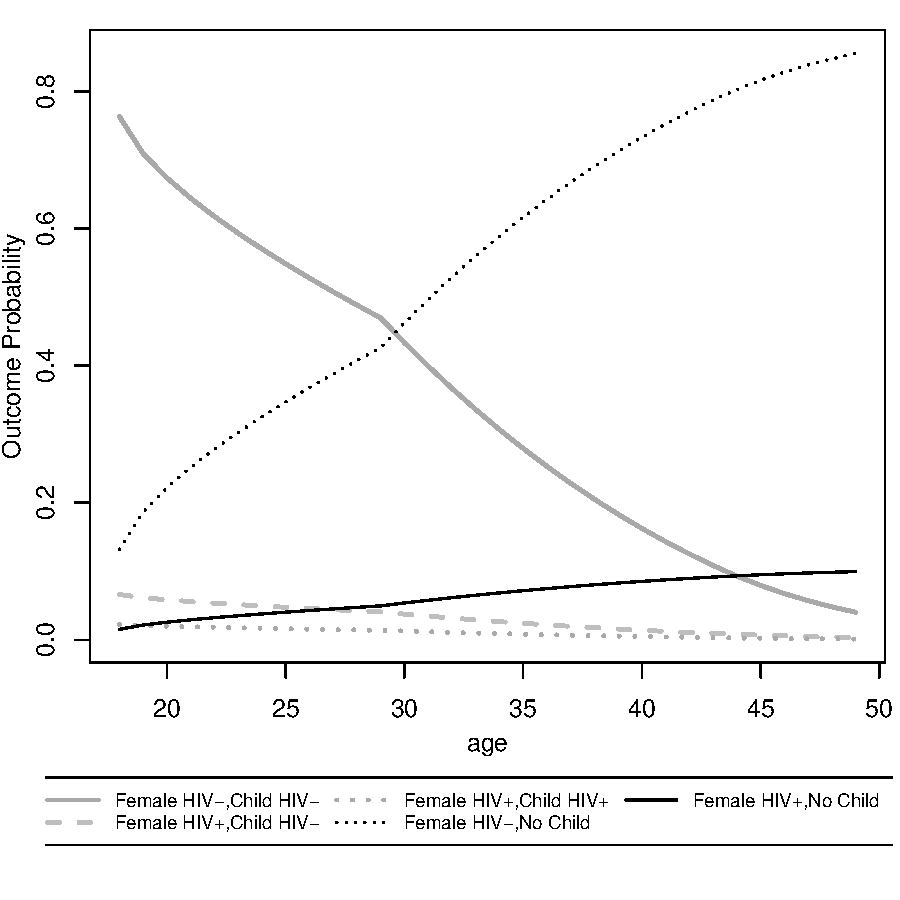
\includegraphics[width=4in]{figures/AgeVary_07Sept2012.pdf}
  \end{center}
  \caption{Outcomes by Varying Age}
  \label{Fig:AgeVary}
\end{figure}

While we know that age strongly influences the chances of conception and delivery, the HIV status of both the mother and child are determined by the other variables.  To better understand how the range of each variable affects the probability of an outcome we use only one binary variable at a time and then vary the parameter over its range.  We use the reference values for the transmissibility ($alpha$), mother to child transmission ($p_{MTCT}$), and the number of sex acts ($N$).  We look at the outcomes for age 20, 30, and 40 years.  In these three instances the age affects both the probability of delivery and probability of conception which causes the most likely outcome to change from the female HIV negative with and HIV negative child at age 20 to female HIV negative with an unsuccessful pregnancy by age 30 and by age 40 this outcome dominates in all instances with the exception of either partner having STIs.  At all three ages, when the multiplicative factor for STIs ($h_{STIs}$) is at very high the transmissibility is multiplied by a rather large factor causing the female to become HIV positive.  Interestingly, as the female ages the most likely outcomes result in an HIV positive status at lower and lower values of the STI factor.  Another interesting observation can be seen at age 40 when the male has late stage HIV; when the multiplicative factor is around the mode (approximately 1.8) the female experiences a decline in the HIV negative and unsuccessful pregnancy status and an increase in becoming HIV positive without a child coupled with a decrease in the probability she will remain HIV negative and also have a child that is HIV negative. 

\begin{figure}[!h]
  \begin{center}
    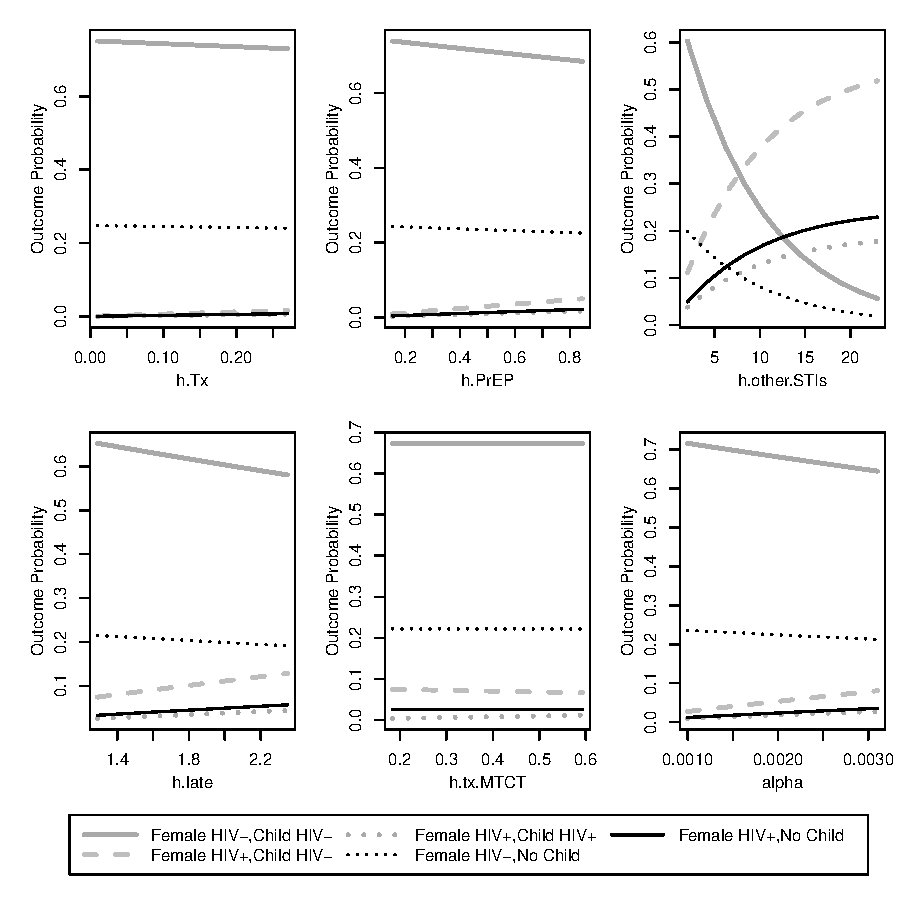
\includegraphics[width=5in]{figures/OnlyVaryParam_Age20_06Sept2012.pdf}
  \end{center}
  \caption{Outcomes by Varying Parameters at Age 20}
  \label{Fig:Vary20}
\end{figure}

\begin{figure}[!h]
  \begin{center}
    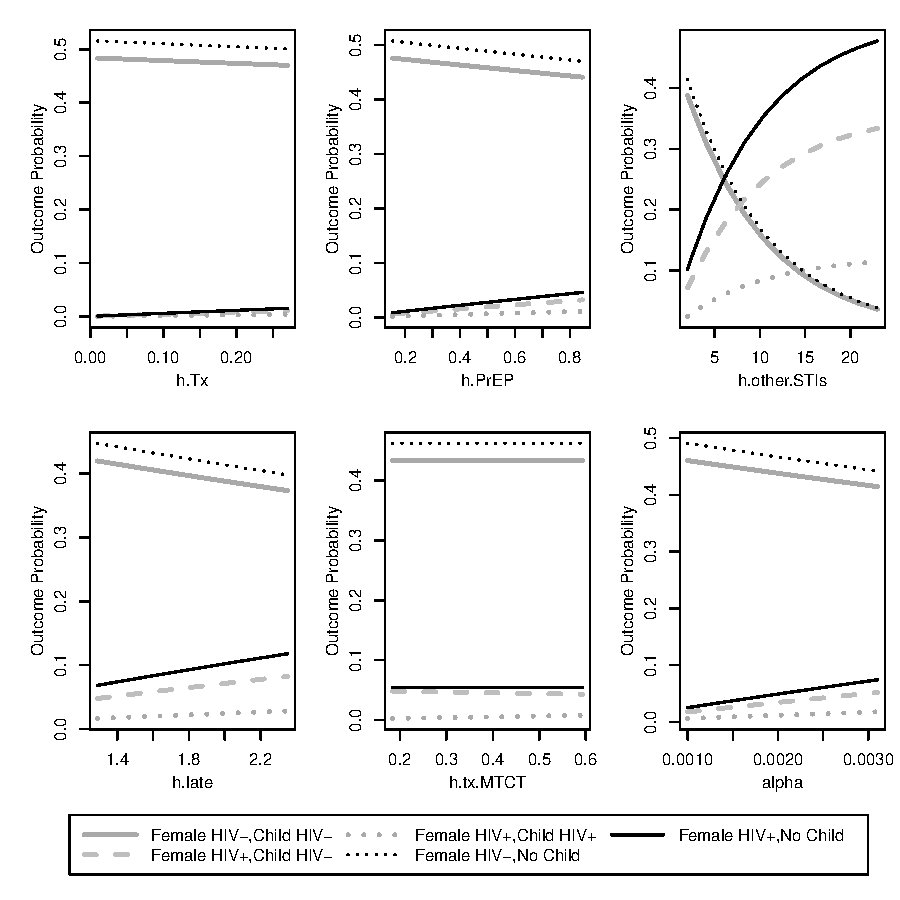
\includegraphics[width=5in]{figures/OnlyVaryParam_Age30_06Sept2012.pdf}
  \end{center}
  \caption{Outcomes by Varying Parameters at Age 30}
  \label{Fig:Vary30}
\end{figure}

\begin{figure}[!h]
  \begin{center}
    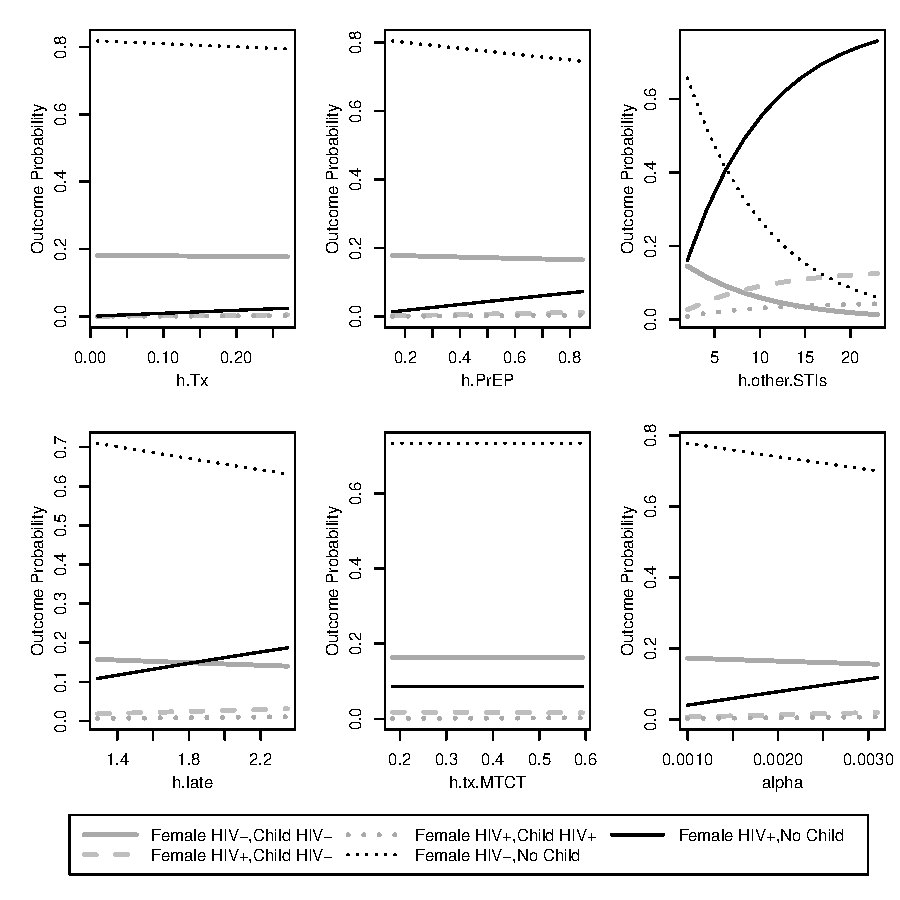
\includegraphics[width=5in]{figures/OnlyVaryParam_Age40_06Sept2012.pdf}
  \end{center}
  \caption{Outcomes by Varying Parameters at Age 40}
  \label{Fig:Vary40}
\end{figure}

We know that the magnitude for the STIs multiplicative factor is the largest and has the largest range of all the variables used to compute the overall transmissibility.  To demonstrate the relative impact of the range on the predicted probabilities we regress the multiplicative factors on each outcome probability.  The multiplicative factor is set to zero when it is "turned off" in a parameter set.  We control for age, number of sex acts, base transmissibility, and mother to child transmission (when there is a successful pregnancy).  Then to obtain the impact of each variable range we set all other variables to their reference values or median values and obtain the predicted probability for each outcome for each variable's minimum and maximum value.  The values displayed in Table ~\ref{tab: rangeImp } are the absolute differences in the predicted probabilities using the minimum and maximum values.  For example for the outcome where a female is HIV negative and has a successful pregnancy, the predicted difference between using the minimum and maximum value for $h_{STIs}$ results in about a 22\% change where as the male being in the later stages of HIV is only about 2.6\% difference, controlling for all other variables.   What we see is that the uncertainty in the $h_{STIs}$ variable can have the greatest impact on the outcome in all five instances.  Keep in mind, that the reported values are for age 30 years, 50 sex acts, and does not account for a mother being on HAART while pregnant.  Changing any of these values will alter the results.

\begin{table}	
\begin{center}
\begin{tabular}{|c|c|c|c|c|c|}
\hline
 & Female HIV-,  & Female HIV+, & Female HIV+, & Female HIV-, & Female HIV+,\\ 
 & Pregnancy Success,& Pregnancy Success,&Pregnancy Success,& Pregnancy& Pregnancy\\ 
 & Child HIV-&Child HIV-&Child HIV+&Unsuccessful&Unsuccessful\\ 
\hline
\hline
Other STIs & 22.40\% & 18.45\% & 3.94\% & 31.87\% & 31.88\%\\ 
Treatment & 18.39\% & 15.04\% & 3.22\% & 24.76\% & 24.90\%\\ 
Late Stage & 2.63\% & 2.14\% & 0.46\% & 3.78\% & 3.82\%\\ 
PrEP & 2.40\% & 2.04\% & 0.44\% & 3.62\% & 3.54\%\\
\hline
\end{tabular}
	\caption{Absolute Change in Predicted Probabilities from the Min and Max Parameter Ranges. \label{tab:rangeImp}}
\end{center}
\end{table}


 \subsection{Influential Variables}
While the previous section tries to explore the impact of the parameter's ranges, this section identifies influential variables; that is regardless of the value, which options have the largest impact on the outcome probabilities (e.g., does having other STIs or the male being on treatment change the probability of an outcome more or less? For a macro perspective we employ linear regression for each of the outcomes.  First we regress the binary variables (whether the male is in the late stage of HIV, if the male is on treatment, if either partner has STIs, if the female is taking PrEP, and if the mother is taking HAART during her pregnancy).  The mother taking HAART is only applicable in the outcomes where she is HIV positive and has a child.  We control for age, transmissibility, the number of sex acts and the mother to child transmissibility (in cases where she is HIV positive and has a child).  In all five outcomes the coefficient for treatment is largest, meaning when a parameter combination has the male on treatment there is largest change in a particular outcome.  Table ~\ref{fig:binaryImp} shows the relative strength of each option; the coefficients from the regressions are divided by the male on treatment coefficient to obtain the relative strength in changing the probability of the particular outcome.   

\begin{table}	
\begin{center}
\begin{tabular}{|c|c|c|c|c|c|}
\hline
 & Female HIV-,  & Female HIV+, & Female HIV+, & Female HIV-, & Female HIV+,\\ 
 & Pregnancy Success,& Pregnancy Success,&Pregnancy Success,& Pregnancy& Pregnancy\\ 
 & Child HIV-&Child HIV-&Child HIV+&Unsuccessful&Unsuccessful\\ 
\hline
\hline
Treatment & 100.00\% & 100.00\% & 100.00\% & 100.00\% & 100.00\%\\ 
Other STIs & 67.82\% & 67.87\% & 67.63\% & 69.00\% & 69.00\%\\ 
PrEP & 25.13\% & 25.06\% & 24.86\% & 25.87\% & 25.87\%\\ 
Late Stage & 20.84\% & 20.72\% & 20.81\% & 22.16\% & 22.16\%\\ 
HAART & - & 11.17\% & 52.02\% & - & -\\
\hline
\end{tabular}
	\caption{Relative Importance of Binary Parameters. \label{tab:binaryImp}}
\end{center}
\end{table}

We have noted that the range for the STI multiplicative factor affects the outcomes the most, yet if all variables were had the same range what would be the impact?  To answer this question we convert all the multiplicative variable ranges to a zero to one scale (if the option is "turned off" we set the value to zero) - this impacts the distribution of the parameters.  To understand the relative impact of each of these variables we regress the parameters, converted to the new ranges, on the outcomes.  Again controlling for age, transmissibility, mother to child transmission, and sex acts.  What is reported in ~\ref{tab: tab:OnePercentIncr} are the regression coefficients which can be interpreted as the effect of a one percent increase in the value of the multiplicative factor on the outcome probability.  While STIs still impact those with successful pregnancies who are HIV positive the most, treatment is more influential for HIV negative females who have successful pregnancies.

\begin{table}	
\begin{center}
\begin{tabular}{|c|c|c|c|c|c|}
\hline
 & Female HIV-,  & Female HIV+, & Female HIV+, & Female HIV-, & Female HIV+,\\ 
 & Pregnancy Success,& Pregnancy Success,&Pregnancy Success,& Pregnancy& Pregnancy\\ 
 & Child HIV-&Child HIV-&Child HIV+&Unsuccessful&Unsuccessful\\ 
\hline
\hline
PrEP & 0.0262 & -0.0278 & -0.0049 & 0.0410 & -0.0396\\ 
Treatment & 0.1682 & -0.1373 & -0.0294 & 0.2259 & -0.2274\\
Other STIs &-0.0240 & 0.1979 & 0.0422 & -0.3437 & 0.3438\\
Late Stage & -0.0260 & 0.0211 & 0.0045 & -0.0372 & 0.0375\\
\hline
\end{tabular}
	\caption{Relative Importance of One Percent Increase of Parameter on Probability of Outcomes. \label{tab:OnePercentIncr}}
\end{center}
\end{table}


\subsection{Regression Trees}
In the previous section, we identified which of the binary variables are of more or less importance in altering the probability within an outcome.  To gain a broader perspective, that is still inline with the results from the previous sections, we use regression trees that recursively dichotomize variables to produce predicted outcomes based upon interacting variables.  These trees are interpreted as follows: in Figure ~\ref{Fig:TreeOutcome1}, a female who is over age 32 and where the male is on treatment and in late stage HIV will have a an estimated probability of 34\% of being HIV negative and have a child that is HIV negative; If the female is less than or equal to 32 years, has more than 21 sex acts, has a male in late stage HIV, and both partners do not have other STIs then she will remain HIV negative and have an HIV negative child with an estimated probability of 46\%.

\begin{figure}[!h]
  \begin{center}
    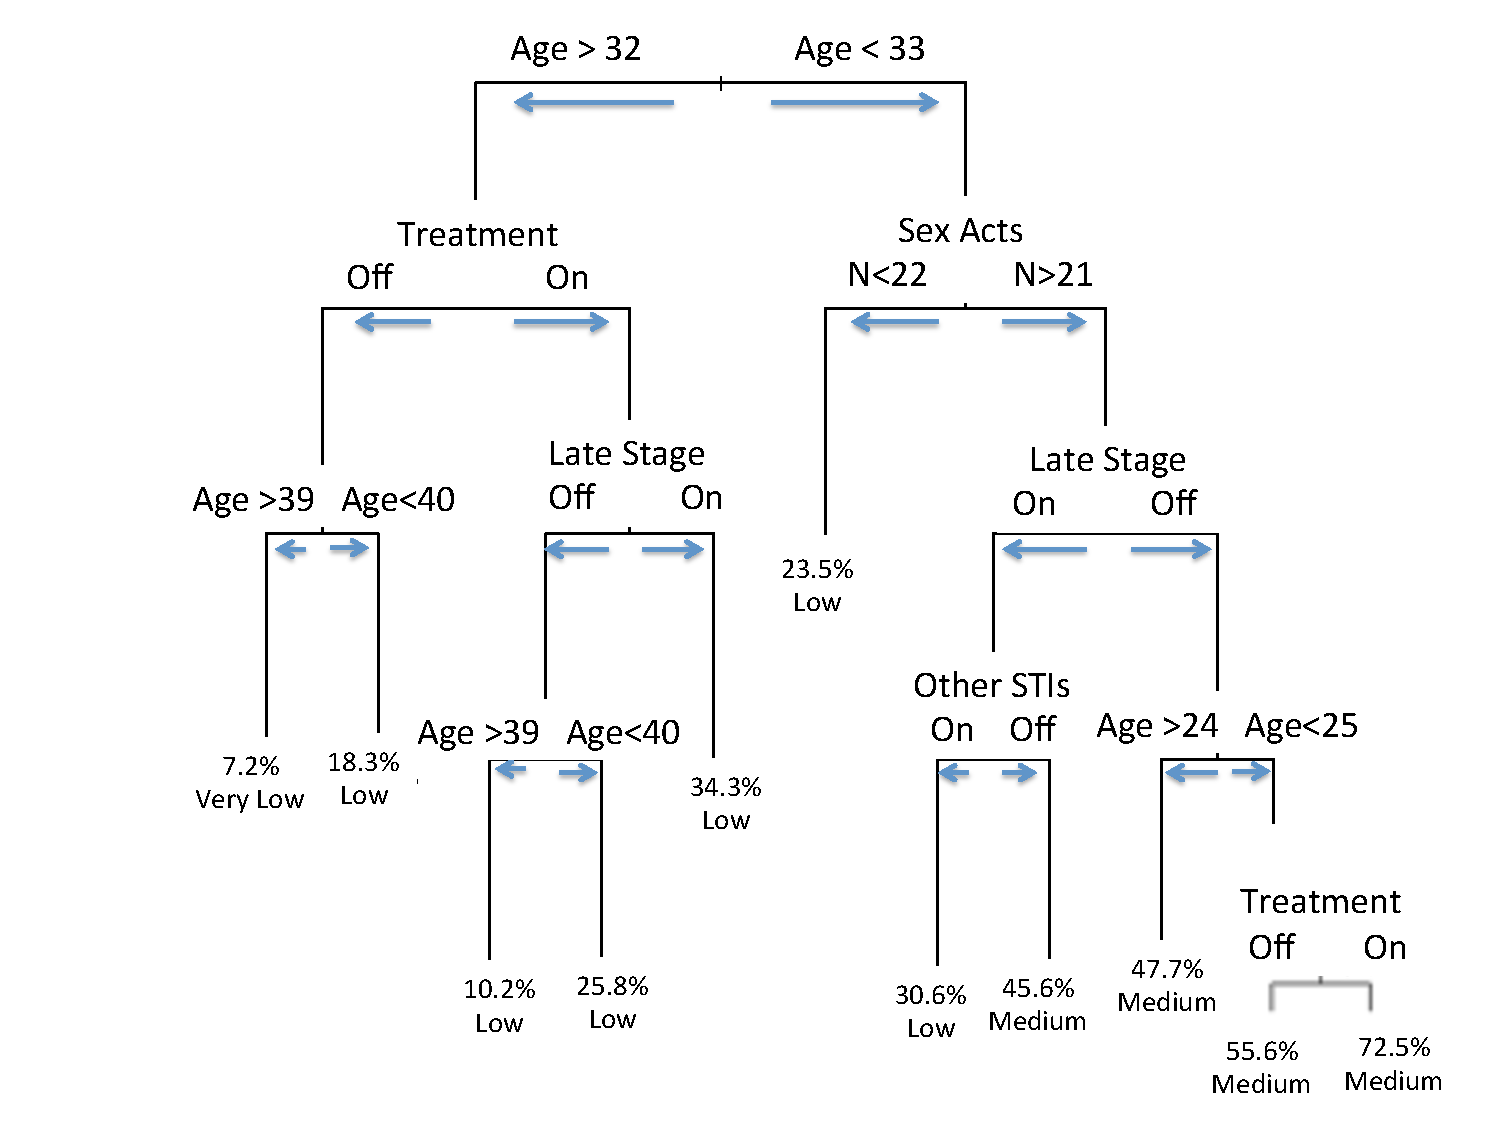
\includegraphics[width=7in]{figures/Tree_Outcome1_09Sept2012.pdf}
  \end{center}
  \caption{Regression Tree for Female HIV-, Child HIV-}
  \label{Fig:TreeOutcome1}
\end{figure}

\begin{figure}[!h]
  \begin{center}
    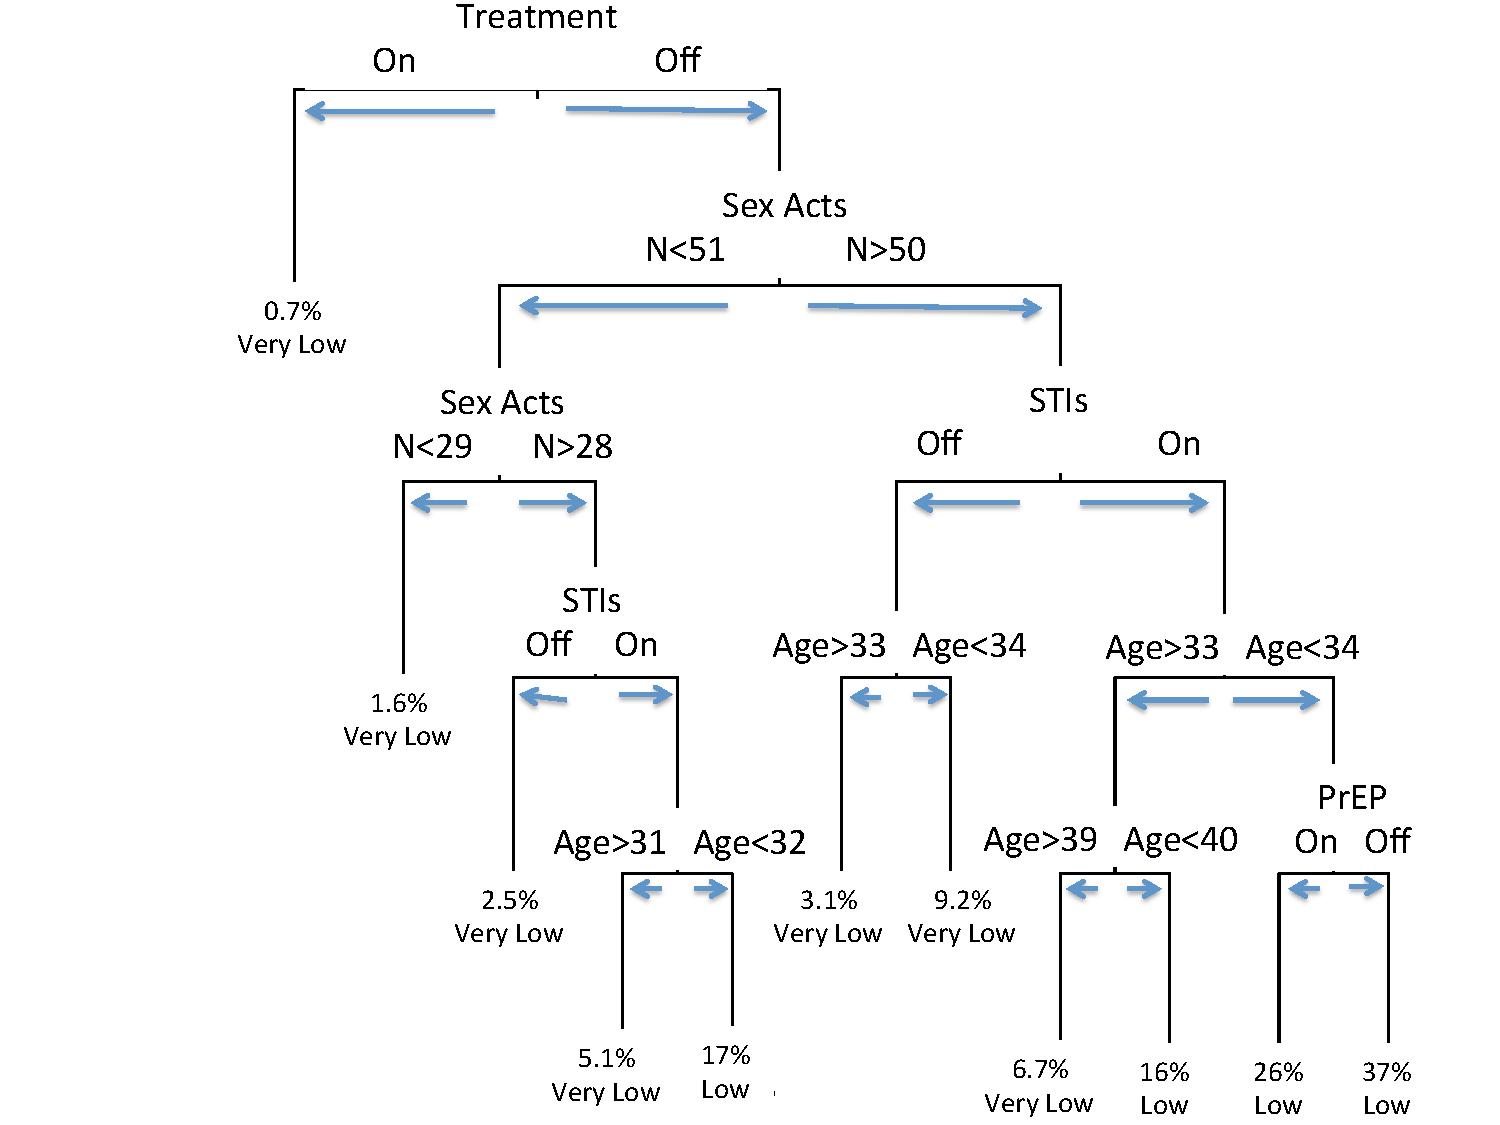
\includegraphics[width=7in]{figures/Tree_Outcome2_09Sept2012.pdf}
  \end{center}
  \caption{Regression Tree for Female HIV+, Child HIV-}
  \label{Fig:TreeOutcome2}
\end{figure}



\newpage


\appendix

\section{The Beta PERT distribution}
\label{sec:PERT}

We run many independent simulations using different combinations of the sampled parameters. For each parameter, we specify a probability distribution that we assume when sampling within its uncertainty range of values. We assume two different probability distributions: uniform and beta PERT (Program Evaluation and Review Technique). For the case that we have large uncertainty in the value of the parameter and any of the values specified in the uncertainty range seems equally likely, we use a uniform distribution. Thus, in this case the specification of a most likely value within this range plays no role in the sampling. A beta PERT distribution instead is used as a continuous approximation to what is normally used, namely a triangular distribution between the minimum and maximum of the uncertainty range and peaking at its most likely value. Typically, sampling from the beta distribution requires minimum and maximum values ($x_{min}$ and $x_{max}$) and two shape parameters, $v$ and $w$. The beta PERT distribution uses the mode or most likely parameter ($x_{mode}$) to generate the shape parameters $v$ and $w$ of a beta distribution. An additional scale parameter $\lambda$ scales the height of the distribution; the default value for this parameter is 4. In the PERT distribution, the mean $\mu$ is calculated
\begin{equation}
	\mu = \frac{x_{min}+x_{max}+\lambda x_{mode}}{\lambda+2},
\end{equation}
and is used to calculate the $v$ and $w$ shape parameters
\begin{equation}
	v = \frac{(\mu-x_{min})(2x_{mode}-x_{min}-x_{max})} {(x_{mode}-\mu)(x_{max}-x_{min}},
\end{equation}
\begin{equation}
	w = \frac{(x_{max}-\mu)(2x_{mode}-x_{min}-x_{max})}{(x_{mode}-\mu)(x_{max}-x_{min}}.
\end{equation} 

\section{Regression Output}
\label{sec:Regression}

XXXX Raff - note sure if I should put tables for all the regression output. XXXX
 
\pagebreak
\bibliographystyle{unsrtnat}
\bibliography{HIV}
\end{document}


